\RequirePackage{plautopatch}
\documentclass[uplatex,dvipdfmx,a4paper,11pt]{jlreq}
\usepackage{bxpapersize}
\usepackage[utf8]{inputenc}
\usepackage{fontenc}
\usepackage{lmodern}
\usepackage{otf}
\usepackage{amsmath}
\usepackage{amssymb}
\usepackage{amsthm}
\usepackage{ascmac}
% \usepackage[hyphens]{url}
\usepackage{mhchem}
\usepackage{siunitx}
\usepackage{physics2}
\usephysicsmodule{ab, ab.braket, doubleprod, diagmat, xmat}
\usepackage{diffcoeff}
% \usepackage{braket}
\usepackage{verbatimbox}
\usepackage{bm}
\usepackage{url}
% \usepackage[dvipdfmx,hiresbb,final]{graphicx}
\usepackage[dvipdfm]{graphicx}
\usepackage{hyperref}
\usepackage{pxjahyper}
\usepackage{tikz}
\usetikzlibrary{cd,intersections,calc,arrows.meta}
\usepackage{listings}
\usepackage{color}
\usepackage{mathtools}
\usepackage{xspace}
\usepackage{xy}
\usepackage{xypic}
%
\title{高温超伝導}
\author{21B00349 宇佐見大希 \\ 共同実験者: 藤木,西澤,出口,宮崎,前山}
\makeatletter
%
\DeclareMathOperator{\lcm}{lcm}
\DeclareMathOperator{\Kernel}{Ker}
\DeclareMathOperator{\Image}{Im}
\DeclareMathOperator{\ch}{ch}
\DeclareMathOperator{\Aut}{Aut}
\DeclareMathOperator{\Log}{Log}
\DeclareMathOperator{\Arg}{Arg}
\DeclareMathOperator{\sgn}{sgn}
%
\newcommand{\CC}{\mathbb{C}}
\newcommand{\RR}{\mathbb{R}}
\newcommand{\QQ}{\mathbb{Q}}
\newcommand{\ZZ}{\mathbb{Z}}
\newcommand{\NN}{\mathbb{N}}
\newcommand{\FF}{\mathbb{F}}
\newcommand{\PP}{\mathbb{P}}
\newcommand{\GG}{\mathbb{G}}
\newcommand{\TT}{\mathbb{T}}
\newcommand{\EE}{\bm{E}}
\newcommand{\rr}{\bm{r}}
\newcommand{\kk}{\bm{k}}
\newcommand{\pp}{\bm{p}}
\newcommand{\calB}{\mathcal{B}}
\newcommand{\calF}{\mathcal{F}}
\newcommand{\ignore}[1]{}
\newcommand{\floor}[1]{\left\lfloor #1 \right\rfloor}
% \newcommand{\abs}[1]{\left\lvert #1 \right\rvert}
\newcommand{\lt}{<}
\newcommand{\gt}{>}
\newcommand{\id}{\mathrm{id}}
\newcommand{\rot}{\curl}
\renewcommand{\angle}[1]{\left\langle #1 \right\rangle}
\newcommand\mqty[1]{\begin{pmatrix}#1\end{pmatrix}}
\newcommand\vmqty[1]{\begin{vmatrix}#1\end{vmatrix}}
\numberwithin{equation}{section}

\let\oldcite=\cite
\renewcommand\cite[1]{\hyperlink{#1}{\oldcite{#1}}}

\let\oldbibitem=\bibitem
\renewcommand{\bibitem}[2][]{\label{#2}\oldbibitem[#1]{#2}}

% theorem環境の設定
% - 冒頭に改行
% - 末尾にdiamond (amsthm)
\theoremstyle{definition}
\newcommand*{\newscreentheoremx}[2]{
  \newenvironment{#1}[1][]{
    \begin{screen}
    \begin{#2}[##1]
      \leavevmode
      \newline
  }{
    \end{#2}
    \end{screen}
  }
}
\newcommand*{\newqedtheoremx}[2]{
  \newenvironment{#1}[1][]{
    \begin{#2}[##1]
      \leavevmode
      \newline
      \renewcommand{\qedsymbol}{\(\diamond\)}
      \pushQED{\qed}
  }{
      \qedhere
      \popQED
    \end{#2}
  }
}
\newtheorem{theorem*}{定理}[section]

\newqedtheoremx{theorem}{theorem*}
\newcommand*\newqedtheorem@unstarred[2]{%
  \newtheorem{#1*}[theorem*]{#2}
  \newqedtheoremx{#1}{#1*}
}
\newcommand*\newqedtheorem@starred[2]{%
  \newtheorem*{#1*}{#2}
  \newqedtheoremx{#1}{#1*}
}
\newcommand*{\newqedtheorem}{\@ifstar{\newqedtheorem@starred}{\newqedtheorem@unstarred}}

\newtheorem{sctheorem*}{定理}[section]
\newscreentheoremx{sctheorem}{sctheorem*}
\newcommand*\newscreentheorem@unstarred[2]{%
  \newtheorem{#1*}[theorem*]{#2}
  \newscreentheoremx{#1}{#1*}
}
\newcommand*\newscreentheorem@starred[2]{%
  \newtheorem*{#1*}{#2}
  \newscreentheoremx{#1}{#1*}
}
\newcommand*{\newscreentheorem}{\@ifstar{\newscreentheorem@starred}{\newscreentheorem@unstarred}}

%\newtheorem*{definition}{定義}
%\newtheorem{theorem}{定理}
%\newtheorem{proposition}[theorem]{命題}
%\newtheorem{lemma}[theorem]{補題}
%\newtheorem{corollary}[theorem]{系}

\newqedtheorem{lemma}{補題}
\newqedtheorem{corollary}{系}
\newqedtheorem{example}{例}
\newqedtheorem{proposition}{命題}
\newqedtheorem{remark}{注意}
\newqedtheorem{thesis}{主張}
\newqedtheorem{notation}{記法}
\newqedtheorem{problem}{問題}
\newqedtheorem{algorithm}{アルゴリズム}

\newscreentheorem*{axiom}{公理}
\newscreentheorem*{definition}{定義}

\renewenvironment{proof}[1][\proofname]{\par
  \normalfont
  \topsep6\p@\@plus6\p@ \trivlist
  \item[\hskip\labelsep{\bfseries #1}\@addpunct{\bfseries}]\ignorespaces\quad\par
}{%
  \qed\endtrivlist\@endpefalse
}
\renewcommand\proofname{証明}

\makeatother

\begin{document}
\maketitle
\tableofcontents
\clearpage

\section{実験目的}
量子力学が目に見える形で現れる超伝導を観察し、液体窒素で超伝導を起こせることを確認して説明できるようになること。

\section{実験原理}
1908 年にオランダのカメリン・オネンスがヘリウムを液化することに成功し、彼はさまざまな物質を冷やしていた。
1911 年に水銀を冷やしたとき約 4.2 \si{K} 以下では電気抵抗が突如ゼロとなった。
これが超伝導の発見となる。
1957 年 Bardeen, Cooper, Schrieffer による BCS 理論によって超伝導の仕組みが解明された。
しかし発見以来 75 年掛けても超伝導転移温度は 20 \si{K} 程度しか上昇しなかった。
1986 年 Bednortz, Muller によって \ce{La_{1-x}Ba_xCuO4} なる銅酸化物や 1987 年 \ce{YBa2Cu3O7} が発見され、爆発的に転移温度が上昇し、液体窒素温度を超えた。

このような高温超電導は共通してペロブスカイト構造 (\ce{ABO3}) で銅酸化物の面が存在する。
例えば今回扱う \ce{YBa2Cu3O_{7-\delta}} は酸素欠損が超伝導の担い手になり、さらに酸素欠損が少ないほど転移温度は高くなるとされている。


\subsection{超伝導の性質}
超伝導の性質で顕著な性質は次の 2 つである。
\begin{itemize}
  \item 完全反磁性 (マイスナー効果)
  \item ゼロ抵抗性
\end{itemize}
まずマイスナー効果について超伝導体はある磁場以下ならば磁束が超伝導内に入らない、つまり
\begin{align}
  \bm{B} = 0
\end{align}
となることが分かっている。
逆にある磁場以上になると部分的に超伝導が壊され磁束が入る現象 (これが起こる超伝導を第二種超伝導といい、そうでないものを第一種超伝導という) がある。
これは入る磁束が量子化されて磁束量子となり、その周りには渦糸と呼ばれる超伝導電流が流れる構造を持ち、互いに相互作用してアブリコソフ格子という六角形の格子を形成する。
これにより結晶の構造欠陥に渦糸が形成されて安定化するというピン止め効果と呼ばれる現象も起こる。

\subsection{熱電対}
熱電対はゼーベック効果によって流れる電流を用いて温度を測る機器である。
基本的には基準点と測りたい対象、気温の 3 つを端子とすることで導線の抵抗の影響を排除できる。
今回の基準点は液体窒素となる。



\section{実験手法}
今回は \ce{YBa2Ca3O7} という YBCO 系の高温の超伝導体を作製し、各性質を調べる。

\subsection{試料の作成}
高温超伝導の試料 \ce{YBa2Ca3O7} を作製する方法として焼結法を用いる。
酸化イットリウム (\ce{Y2O3}), 炭酸バリウム (\ce{BaCO3}), 酸化銅 (\ce{CuO}) を用いて 930 \si{\degreeCelsius} で次の反応を起こす。
\begin{align}
  \ce{1/2Y2O3 + 2BaCO3 + 3CuO -> YBa2Cu3O_{7-\delta} + 2CO2}
\end{align}
ここではモル比が $\ce{Y}:\ce{Ba}:\ce{Cu} = 1:2:3$ となるように計 4.000 \si{g} となるように秤量する。
各物質の秤量を実際に計算すると表 \ref{table:mixture} のようになる。
\begin{table}
  \centering
  \begin{tabular}{|c|c|c|c|}
    \hline
    物質                           & 分子量    & モル数                            & 重さ           \\
    \hline
    \hline
    \ce{Y2O3}                    & 225.81 & $2.68\times 10^{-3}$ \si{mol}  & 0.605 \si{g} \\
    \ce{BaCO3}                   & 197.34 & $10.72\times 10^{-3}$ \si{mol} & 2.116 \si{g} \\
    \ce{CuO}                     & 79.55  & $16.08\times 10^{-3}$ \si{mol} & 1.279 \si{g} \\
    \hline
    \ce{1/2Y2O3 + 2BaCO3 + 3CuO} & 746.24 & $5.36\times 10^{-3}$ \si{mol}  & 4.000 \si{g} \\
    \hline
  \end{tabular}
  \caption{混合比率}
  \label{table:mixture}
\end{table}

これらを乳鉢に入れて乳棒で撹拌しながら粉砕し、電気炉で 1 時間仮焼きをしてまた粉砕する。
その後プレス機で約 1 \si{ton/cm^2} の圧力でプレスしてペレット状の試料を 2 つ作る。
それらを再度 6 時間本焼きして徐冷で室温に戻す。
使い終わったら希塩酸を用いて乳鉢や乳棒を洗浄する。その廃液は流しに流さず、容器に入れて保管する。


\subsection{磁気浮上効果の観察}
ネオジム磁石 (表面磁束密度は約 0.3 \si{T}) の上に冷却した試料を乗せる。
これにはゼロ磁場冷却と磁場中冷却の 2 通りを試し、マイスナー効果およびピン止め効果が現れていることを確認する。
またアルミホイールで覆うなどの保温することで持続時間を伸ばす方法を考える。


\subsection{X 線回折による物質の同定}
作成した試料を X 線の回折スペクトルを測定することでどのような物質が生成されているかを調べる。

X 線回折装置の全体としては電子銃から発射される電子を \ce{Mo} に当て、その放射として出る K$\alpha$ 線を用いて X 線を発射し、試料に当てて回折スペクトルを調べる。
回折の仕組みについて詳しく説明する。
この X 線は試料に当たるとそれを構成する原子の電子によって散乱される。 (Thomson 散乱)
\begin{align}
  A(\bm{K}) & = \int \rho(\rr)\exp(-i\bm{K}\cdot\rr)\dl{\rr}                                                                                                                                         \\
            & = \sum_{n_1 = 0}^{N_1 - 1}\sum_{n_2 = 0}^{N_2 - 1}\sum_{n_3 = 0}^{N_3 - 1}\exp(-i\bm{K}\cdot(n_1\bm{a}_1 + n_2\bm{a}_2 + n_3\bm{a}_3))\int_{UC}\rho(\rr)\exp(-i\bm{K}\cdot\rr)\dl{\rr} \\
            & = G(\bm{K}) F(\bm{K})
\end{align}
\begin{align}
  G(\bm{K}) & = \sum_{n_1 = 0}^{N_1 - 1}\sum_{n_2 = 0}^{N_2 - 1}\sum_{n_3 = 0}^{N_3 - 1}\exp(-i\bm{K}\cdot(n_1\bm{a}_1 + n_2\bm{a}_2 + n_3\bm{a}_3))                                                                                                                       \\
            & = \exp\ab(-i\frac{N_1 - 1}{2}\bm{K}\cdot\bm{a}_1)\frac{\sin\frac{N_1\bm{K}\cdot\bm{a}_1}{2}}{\sin\frac{\bm{K}\cdot\bm{a}_1}{2}}\exp\ab(-i\frac{N_2 - 1}{2}\bm{K}\cdot\bm{a}_2)\frac{\sin\frac{N_2\bm{K}\cdot\bm{a}_2}{2}}{\sin\frac{\bm{K}\cdot\bm{a}_2}{2}} \\
            & \times \exp\ab(-i\frac{N_3 - 1}{2}\bm{K}\cdot\bm{a}_3)\frac{\sin\frac{N_3\bm{K}\cdot\bm{a}_3}{2}}{\sin\frac{\bm{K}\cdot\bm{a}_3}{2}}                                                                                                                         \\
  F(\bm{K}) & = \int_{UC}\rho(\rr)\exp(-i\bm{K}\cdot\rr)\dl{\rr}
\end{align}
$G(\bm{K})$ の絶対値が大きくなる条件は次のようになる。
\begin{align}
  \bm{K}\cdot\bm{a}_1 = 2\pi m_1, \quad
  \bm{K}\cdot\bm{a}_2 = 2\pi m_2, \quad
  \bm{K}\cdot\bm{a}_3 = 2\pi m_3
\end{align}
これは逆格子ベクトルの定義と等しいから $\bm{K} = \bm{G}_m$ となる。
これを Laue の条件という。
また $|\bm{K}| = |\bm{G}_m| = 2|\kk|\sin\theta = \frac{2\pi}{d}$ とおくと Bragg 条件
\begin{align}
  2d\sin\theta = n\lambda
\end{align}
となる。

他にも 3 次元結晶 ($a\perp b\perp c$) で Miller 指数 $[h\ k\ l]$ における面間隔 $d$ は次式を満たす。
\begin{align}
  \frac{1}{d^2} & = \ab(\frac{h}{a})^2 + \ab(\frac{k}{b})^2 + \ab(\frac{l}{c})^2
\end{align}
これより次のような式が成り立つ。
\begin{align}
  \sin\theta & = \frac{1}{2}\sqrt{\ab(\frac{\lambda}{a})^2h^2 + \ab(\frac{\lambda}{b})^2k^2 + \ab(\frac{\lambda}{c})^2l^2}
\end{align}
入射と回折 X 線のなす角 $2\theta$ が X 線回折装置によって出力される。
具体的な値として X 線の波長は $\lambda = 1.541$ \si{\AA}, あり得る物質の結晶格子の格子定数は表 \ref{table:crystal structure} にとなる。
\begin{table}
  \centering
  \begin{tabular}{|c|c|c|c|}
    \hline
    物質             & a 軸 (\si{\AA}) & b 軸 (\si{\AA}) & c 軸 (\si{\AA}) \\
    \hline
    \hline
    \ce{YBa2Cu3O7} & 3.818          & 3.888          & 11.80          \\
    \ce{Y2BaCuO5}  & 7.132          & 12.181         & 5.658          \\
    \ce{CuO}       & 4.684          & 3.425          & 5.129          \\
    \ce{Y2O3}      & 10.605         & 10.605         & 10.605         \\
    \hline
  \end{tabular}
  \caption{アニールで得られうる物質の結晶構造}
  \label{table:crystal structure}
\end{table}



\subsection{電気抵抗の測定}
四端子法を用いて電流と電圧を測り、電気抵抗を測定する。

まず試料を小さくカットする。
その試料の 4 ヶ所に銅線を銀ペーストを用いて付け、それぞれのリード線をホルダーにはんだ付けする。
端子の部分にテフロンテープを巻いて絶縁してからアルミホイールで包んで保温する。
電圧から定常的な電流に変換して端子へ繋ぎ、電圧を測定する。
これを熱電対で試料周辺の温度を測りながら液体窒素の中にゆっくり浸けて温度と抵抗の関係をプロットする。

\begin{figure}[htbp]
  \centering
  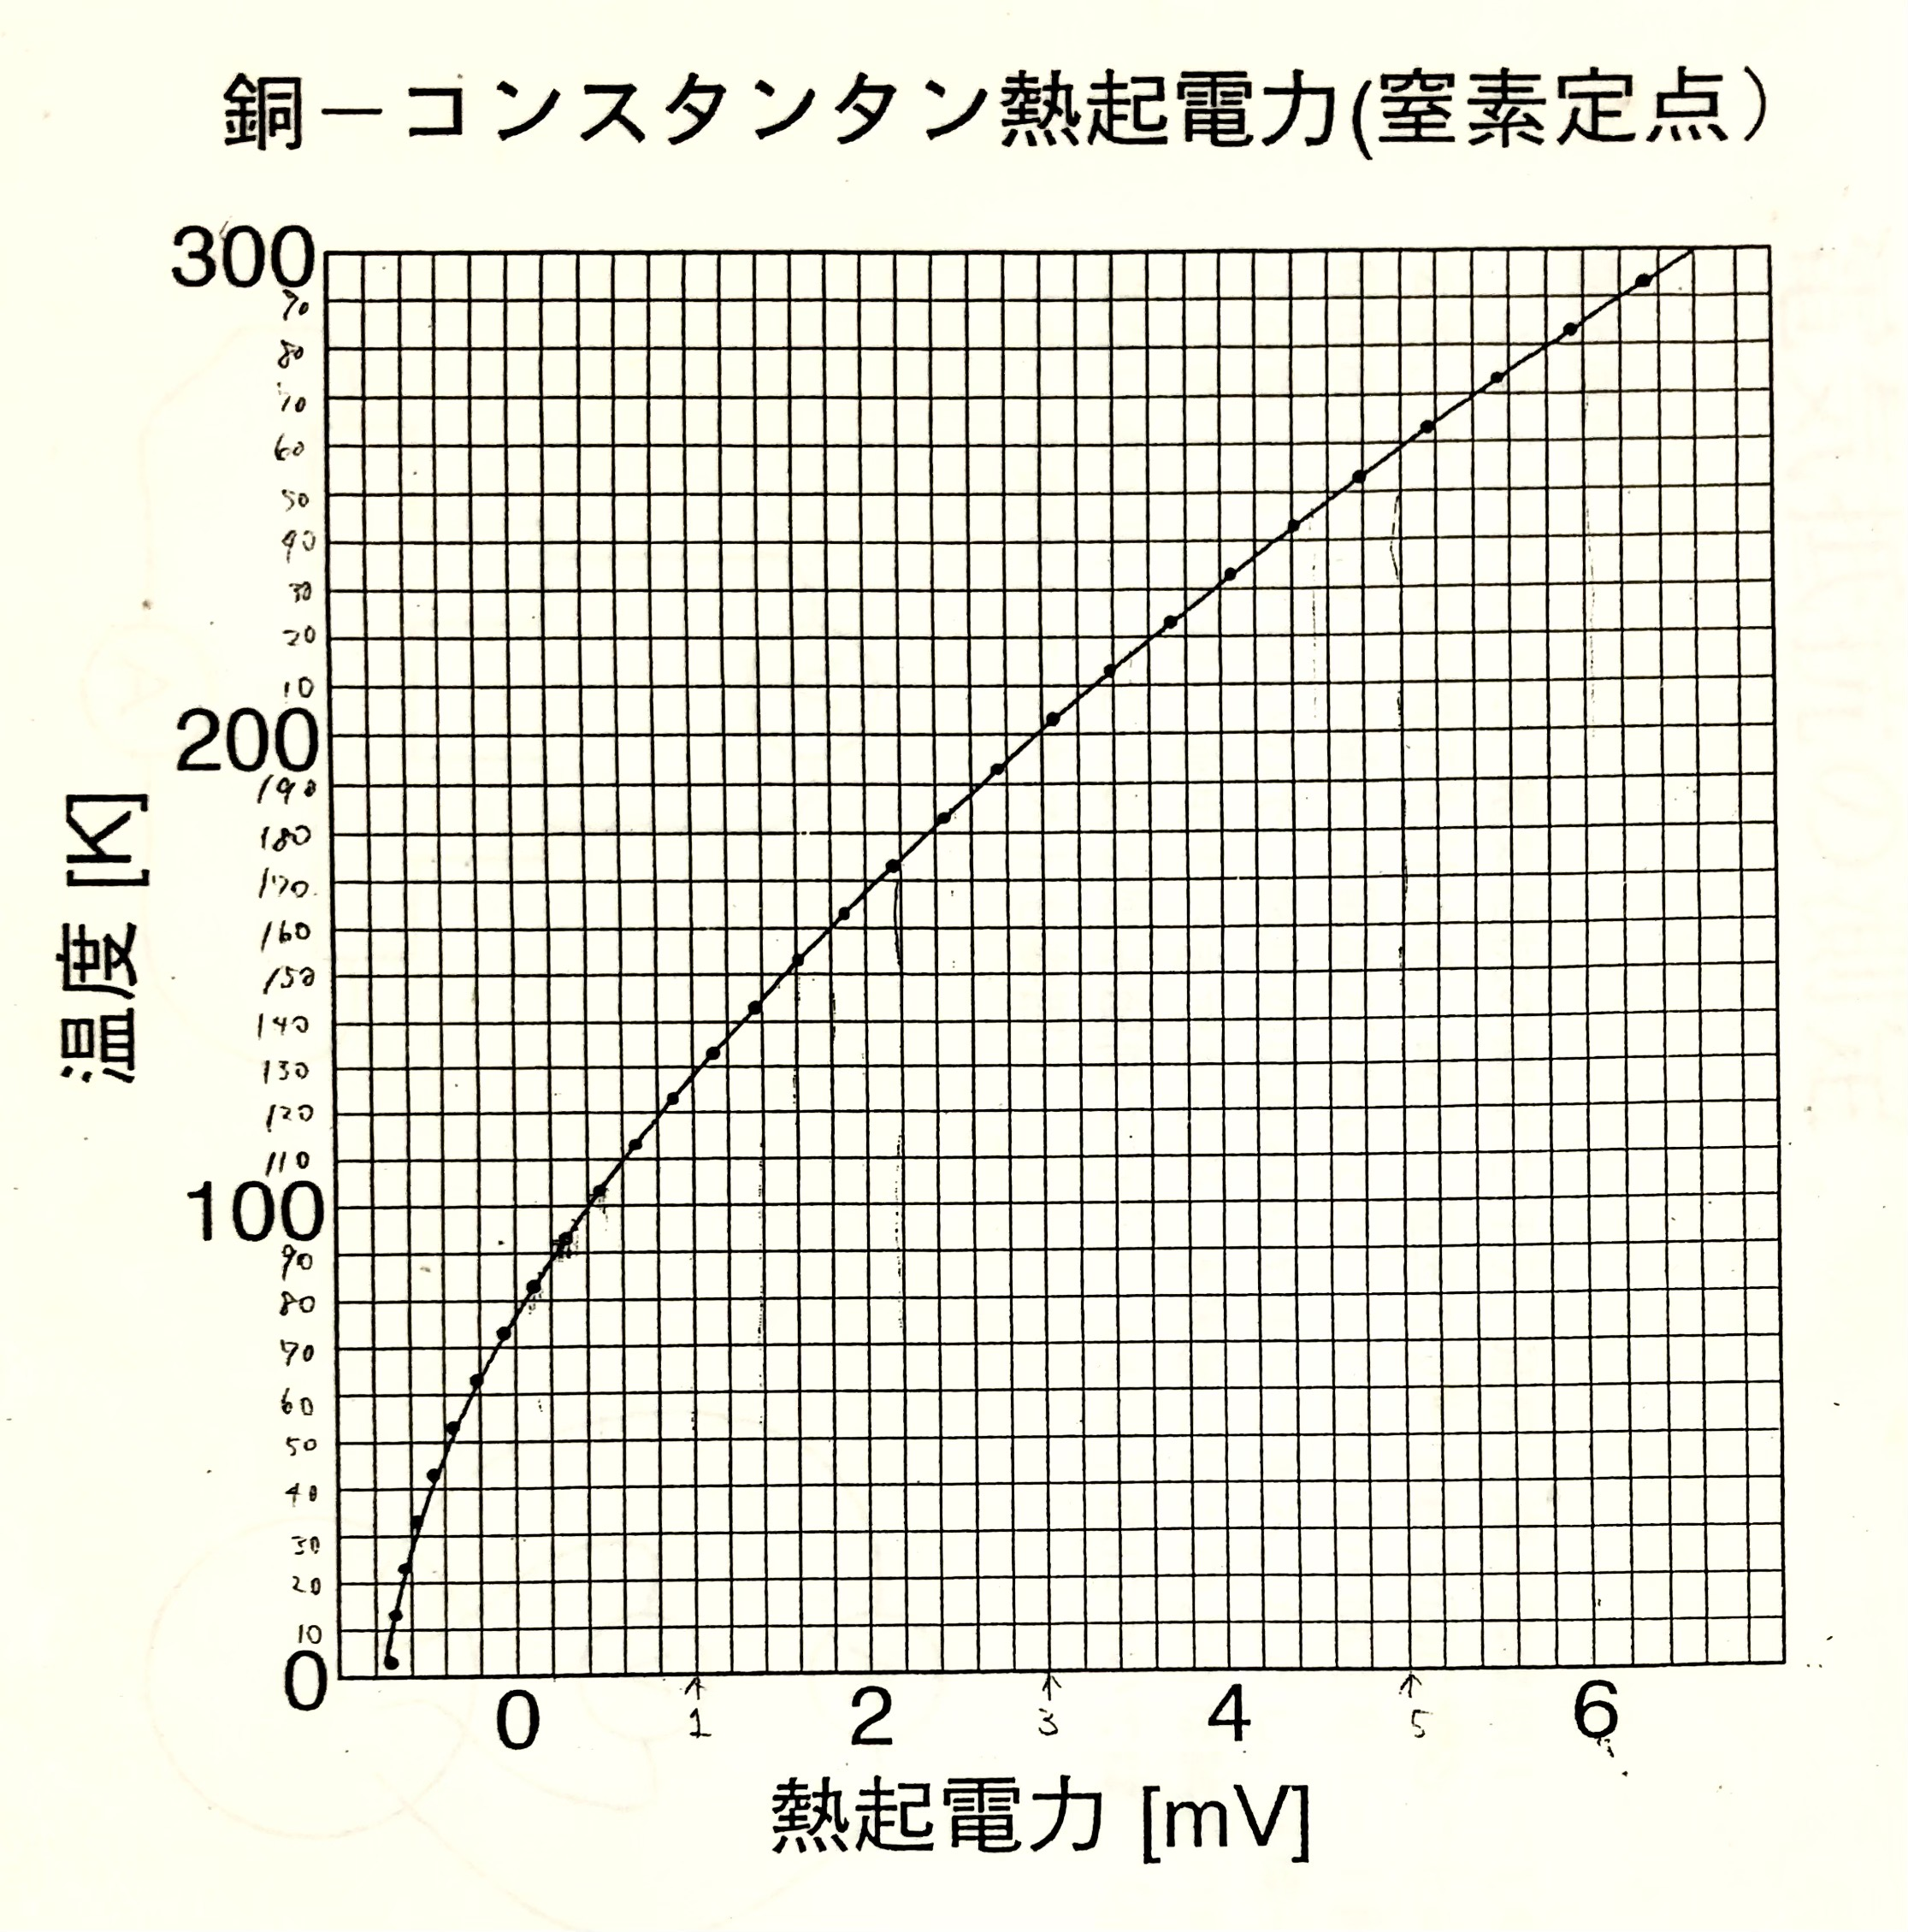
\includegraphics[width=10cm]{./assets/YBCO_thermocouple.jpg}
  \caption{熱電対の出力と温度の関係}
  \label{fig:thermo}
\end{figure}
抵抗率 $\rho$ については抵抗 $R$ に対して断面積 $S$ と距離 $\ell$ を用いて次のように定義される。
\begin{align}
  \rho = R\frac{S}{\ell} = \frac{V}{I}\frac{S}{\ell}
\end{align}
ここでは電流 70.00 \si{mA} を流し、今回の試料については断面積 $2.4\si{mm} \times 4.1\si{mm}$, 距離 0.8 \si{mm} となった。



\subsection{交流帯磁率の測定}
2 つのコイルの相互インダクタンスの変化を測ることで試料の帯磁率を調べる。
\begin{align}
  V_{osc} & = V_0\exp(i\omega t)                              \\
  I       & = C_0V = C_0V_0\exp(i\omega t)                    \\
  V_{out} & = -M\diff{I}{t} = -i\omega C_0V_0M\exp(i\omega t)
\end{align}
最初にコイル 1 とコイル 2 の電圧 $V_1, V_2$ が等しくなるように調整しておく。
超伝導は磁束が入らない ($\bm{B} = 0$) から帯磁率は $\chi = -1$ となる。
コイル内に試料を入れることで相互インダクタンスが体積比で変化すると考える。
このときコイル内の体積に対して超伝導化した試料の体積の比 $v/V$ がわかる。
\begin{align}
  M           & = \mu_0(1 + \chi)n_1n_2l_2S_1                                                                            \\
  V_1' - V_2  & = -i\omega C_0V_{01}\ab\{\ab(\ab(1 - \frac{v}{V})M_{01} + \frac{v}{V}\times 0) - M_{01}\}\exp(i\omega t) \\
              & = i\omega C_0V_{01}M_{01}\frac{v}{V}\exp(i\omega t)                                                      \\
  \frac{v}{V} & = \frac{\mathrm{Im} (V_1' - V_2)}{\omega C_0V_{01}M_{01}}
\end{align}
コイルは巻数はどちらも 1000 回であり, コイルは長さ 45 \si{mm}, 直径 20 \si{mm} の円柱形であり, 交流周波数は 110 \si{Hz} とする。




\section{実験結果}
\subsection{磁気浮上効果の観察}
今回作製した 2 つの試料を用いて磁気浮上効果を観察した。

まず図 \ref{fig:mag1} のように磁石を配置したときに磁気浮上効果が確認できた。
磁気浮上効果により浮上した高さはどちらも 6 \si{mm} 程度で持続時間はそれぞれ 7 \si{s}, 13 \si{s} であった。
またアルミホイールを巻いて試料の温度を上がらないようにした状態のとき、高さは変わらず持続時間がそれぞれ 16 \si{s}, 25 \si{s} と倍程度長くなった。

次に図 \ref{fig:mag2} のようなレール状に配置して冷却した試料を置いて力を加えたとき試料は滑走した。
曲がるときに試料は中心に対して向きが変わらないように曲がった。

さらに試料を回転させながら磁束中に入れると静止した。

磁場中冷却すると試料内の磁束の向きが固定化され、裏返すと反発した。

\begin{figure}[htbp]
  \begin{minipage}[b]{0.5\linewidth}
    \centering
    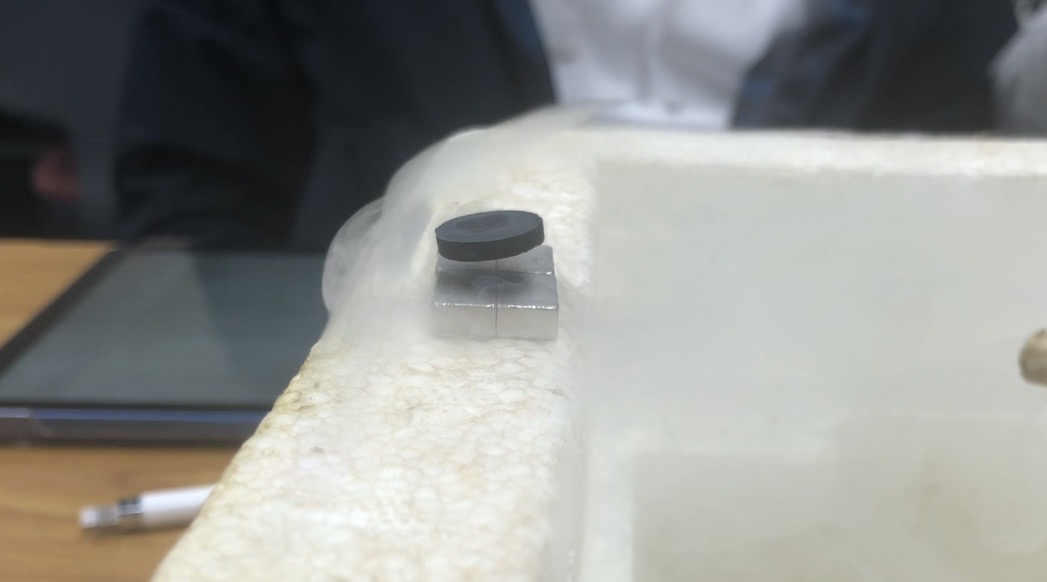
\includegraphics[keepaspectratio, width=8cm]{./assets/YBCO_image2.jpg}
  \end{minipage}
  \begin{minipage}[b]{0.5\linewidth}
    \centering
    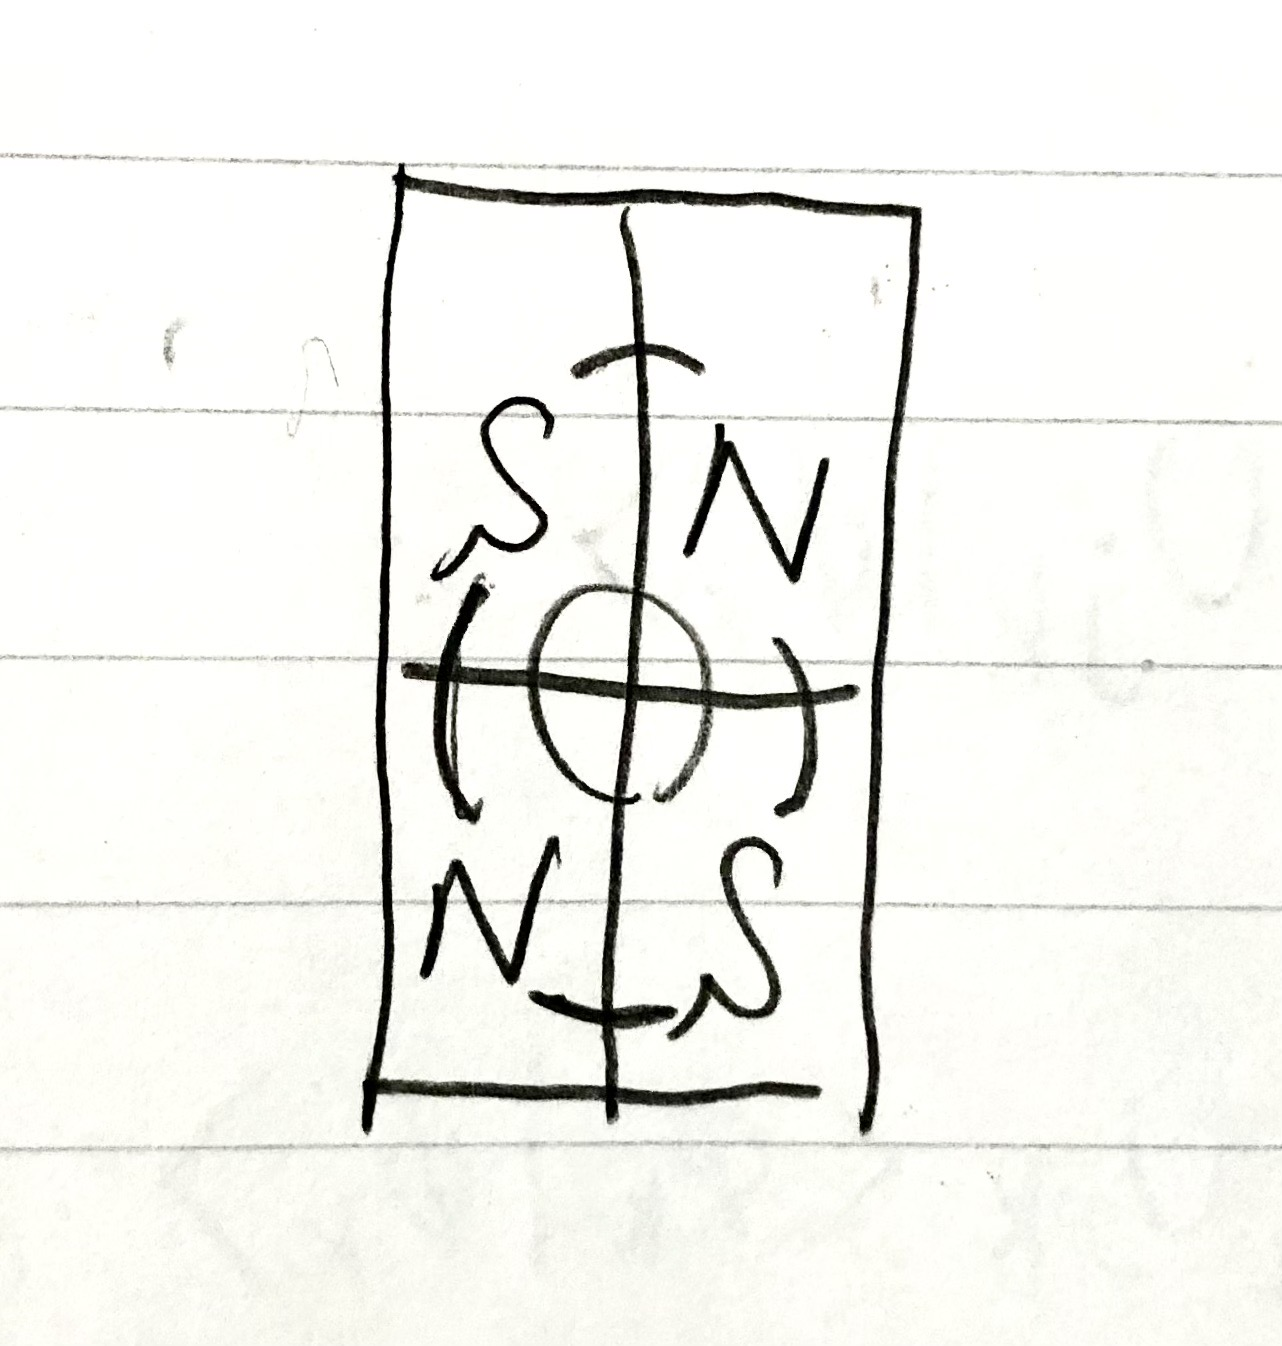
\includegraphics[keepaspectratio, width=4cm]{./assets/YBCO_magnet.jpg}
  \end{minipage}
  \caption{磁気浮上効果1}
  \label{fig:mag1}
\end{figure}
\begin{figure}[htbp]
  \begin{minipage}[b]{0.5\linewidth}
    \centering
    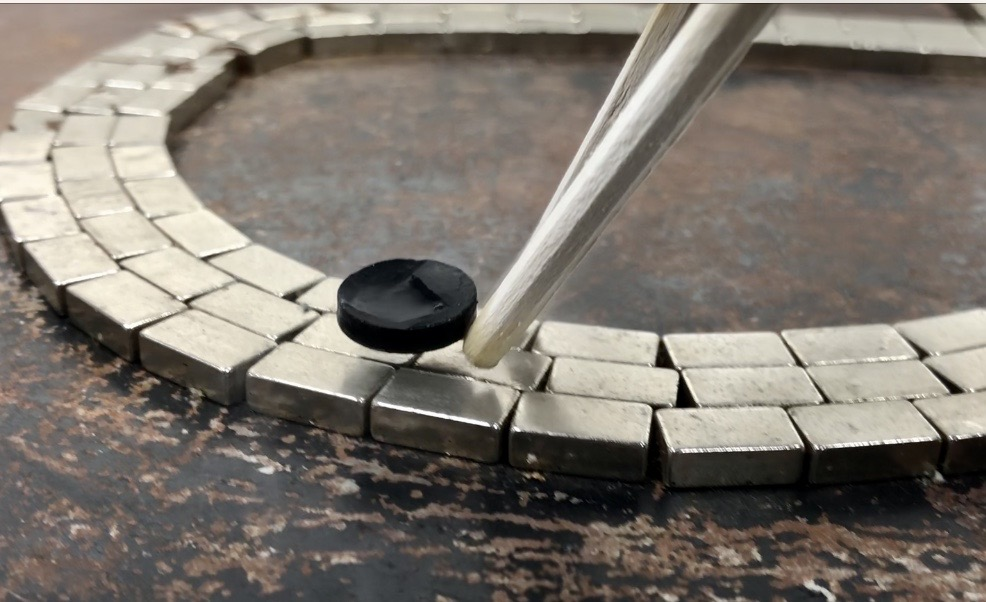
\includegraphics[keepaspectratio, width=7cm]{./assets/YBCO_image3.jpg}
  \end{minipage}
  \begin{minipage}[b]{0.5\linewidth}
    \centering
    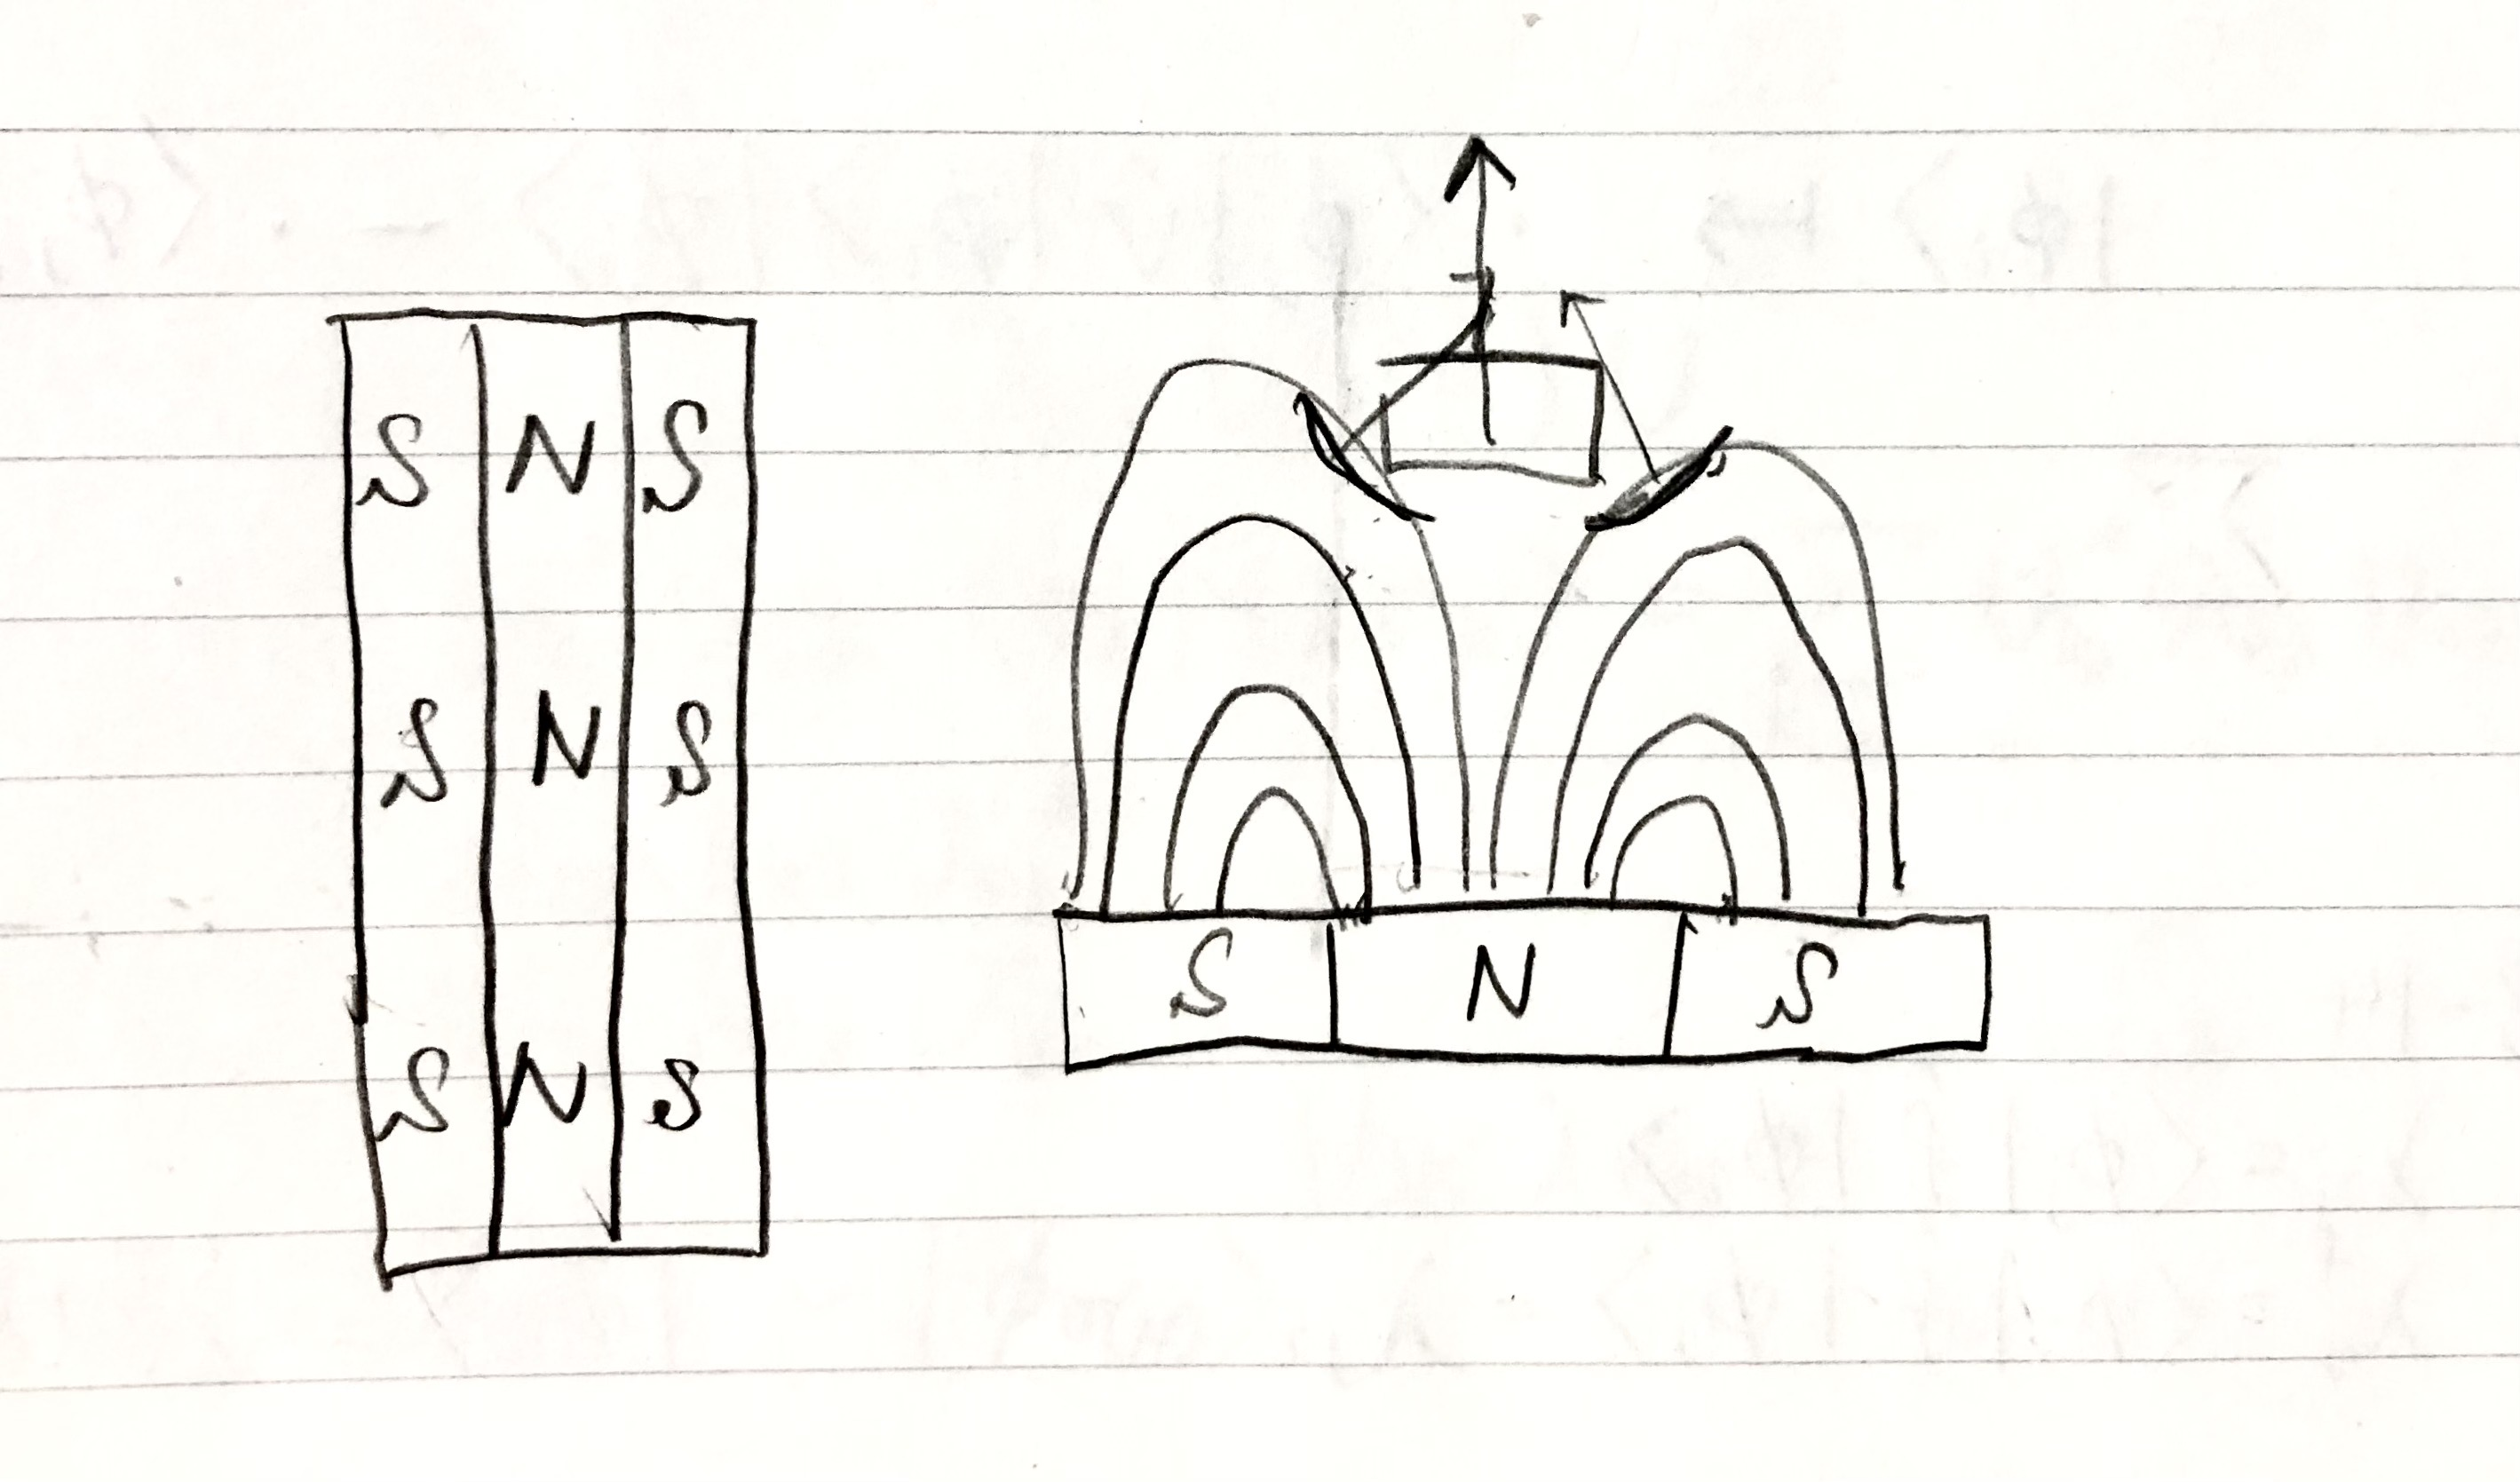
\includegraphics[keepaspectratio, width=6cm]{./assets/YBCO_mag_line.jpg}
  \end{minipage}
  \caption{磁気浮上効果2}
  \label{fig:mag2}
\end{figure}

\subsection{X 線回折による物質の同定}
X 線回折装置を用いて回折による角度に対する強度は図 \ref{fig:xray} のようになる。
\begin{figure}[htbp]
  \centering
  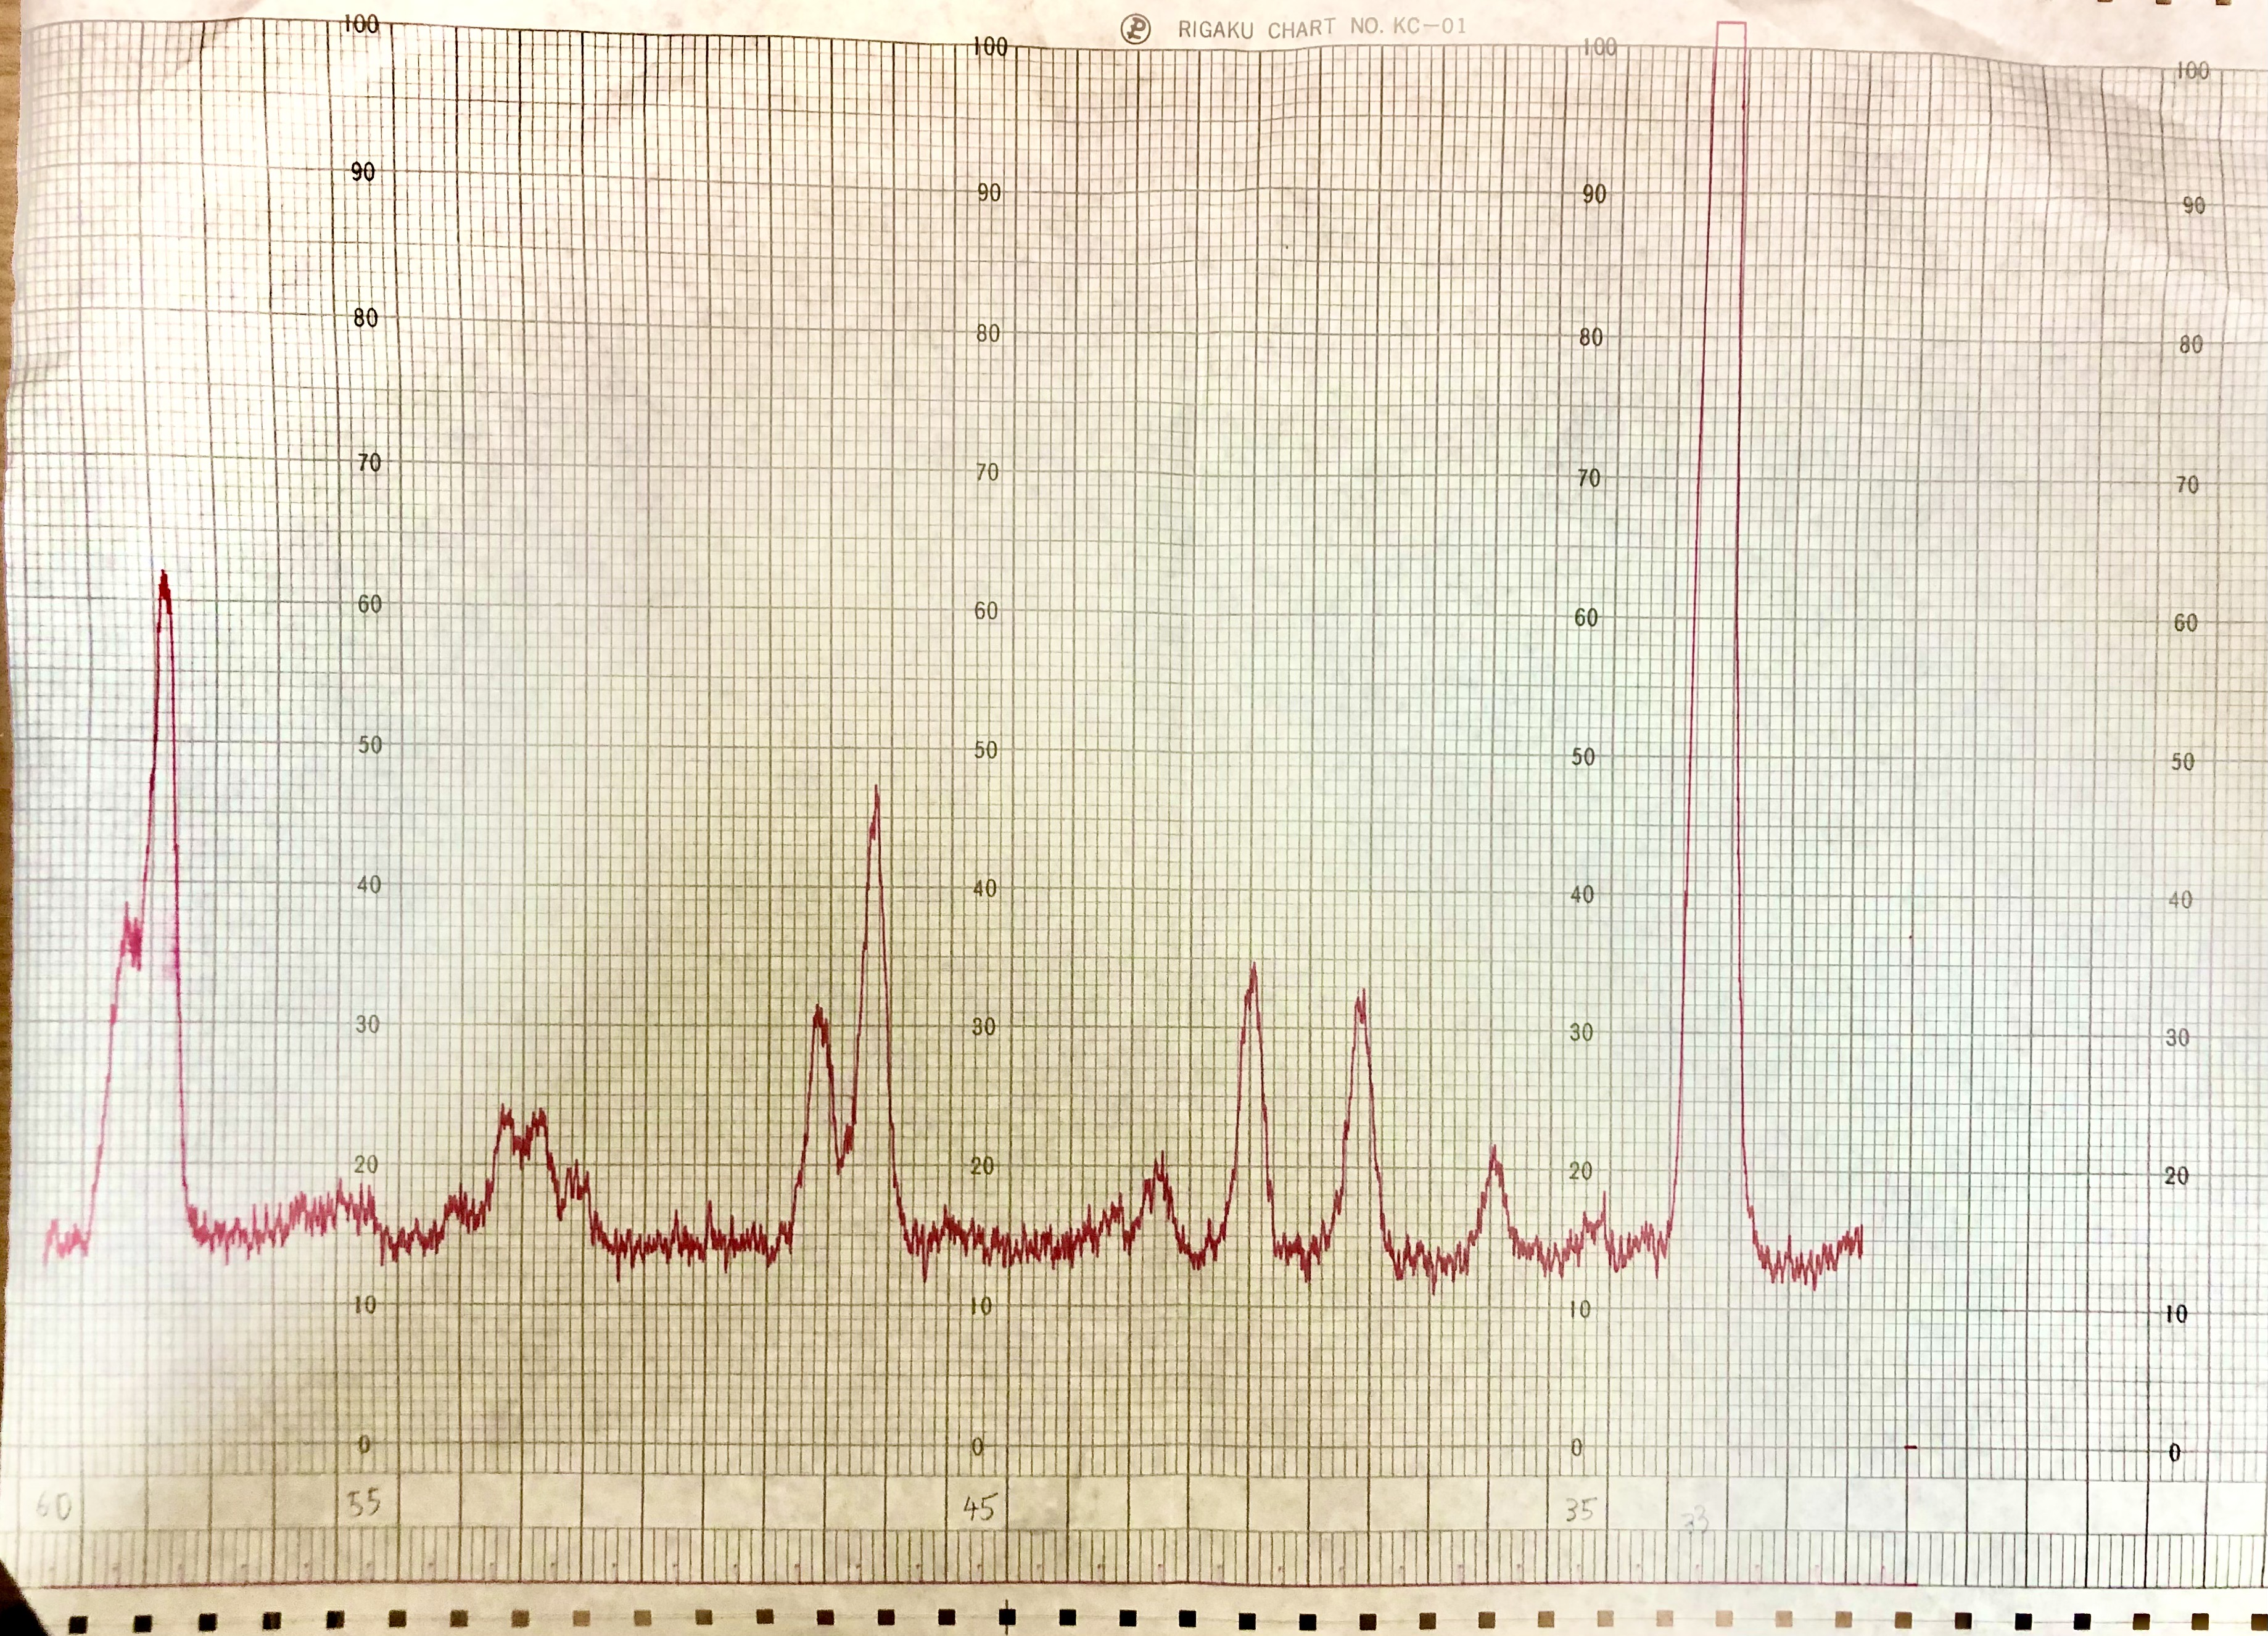
\includegraphics[width=10cm]{./assets/YBCO_xray.jpg}
  \caption{X 線回折}
  \label{fig:xray}
\end{figure}

角度と対応した合成される可能性のある結晶の Miller 指数を表 \ref{table:miller} のようにまとめた。

\begin{table}
  \centering
  \begin{tabular}{|c|c|c|c|c|c|}
    \hline
    角度 $2\theta$          & 強度         & \ce{YBa2Cu3O7}            & \ce{Y2BaCuO5}             & \ce{CuO}                  & \ce{Y2O3}                            \\
    \hline
    \hline
    \ang{32.8}            & 100 $\leq$ & $[1\ 1\ 0]$ (\ang{32.86}) & $[0\ 1\ 2]$ (\ang{32.47}) & $[1\ 1\ 0]$ (\ang{32.36}) &                                      \\
    \ang{34.6}            & 18         &                           & $[1\ 1\ 2]$ (\ang{34.89}) &                           & $[2\ 2\ 3]$ (\ang{34.86})            \\
    \ang{36.5}            & 22         & $[1\ 1\ 2]$ (\ang{36.30}) & $[0\ 5\ 0]$ (\ang{36.87}) &                           &                                      \\
    \ang{38.6}            & 33         & $[1\ 0\ 4]$ (\ang{38.54}) & $[3\ 1\ 0]$ (\ang{38.56}) & $[2\ 0\ 0]$ (\ang{38.42}) & $[1\ 2\ 4]$ (\ang{38.90})            \\
    \ang{40.4}            & 35         & $[1\ 1\ 3]$ (\ang{40.25}) & $[0\ 5\ 1]$ (\ang{40.28}) &                           &                                      \\
    \ang{42.0}            & 21         &                           & $[2\ 4\ 1]$ (\ang{42.14}) &                           & $[2\ 2\ 4]$ (\ang{41.70})            \\
    \ang{46.7}            & 48         & $[0\ 2\ 0]$ (\ang{46.70}) & $[2\ 3\ 2]$ (\ang{46.67}) & $[2\ 1\ 0]$ (\ang{46.98}) & $[1\ 2\ 5]$ (\ang{46.90})            \\
    \ang{47.7}            & 31         & $[2\ 0\ 0]$ (\ang{47.61}) &                           &                           &                                      \\
    \ang{51.5}-\ang{51.8} & 20         &                           & $[4\ 1\ 0]$ (\ang{51.79}) &                           & $[2\ 2\ 4]$ (\ang{51.69})            \\
    \ang{52.3}            & 24         & $[1\ 0\ 6]$ (\ang{52.30}) & $[1\ 2\ 3]$ (\ang{52.35}) &                           & $[0\ 1\ 6]$ (\ang{52.46})            \\
    \ang{52.8}            & 24         & $[1\ 2\ 0]$ (\ang{52.82}) &                           & $[2\ 0\ 2]$ (\ang{52.92}) &                                      \\
    \ang{58.3}            & 62         & $[1\ 2\ 3]$ (\ang{58.16}) &                           &                           & $[2\ 4\ 5], [0\ 3\ 6]$ (\ang{58.34}) \\
    \ang{58.9}            & 39         & $[2\ 1\ 3]$ (\ang{58.74}) & $[4\ 3\ 1]$ (\ang{58.84}) & $[3\ 0\ 0]$ (\ang{59.14}) & $[1\ 3\ 6]$ (\ang{59.05})            \\
    \hline
  \end{tabular}
  \caption{Miller 指数}
  \label{table:miller}
\end{table}



\subsection{電気抵抗の測定}
熱電対の出力と電圧の関係は図 \ref{fig:resistance} のようになった。
\begin{figure}[htbp]
  \centering
  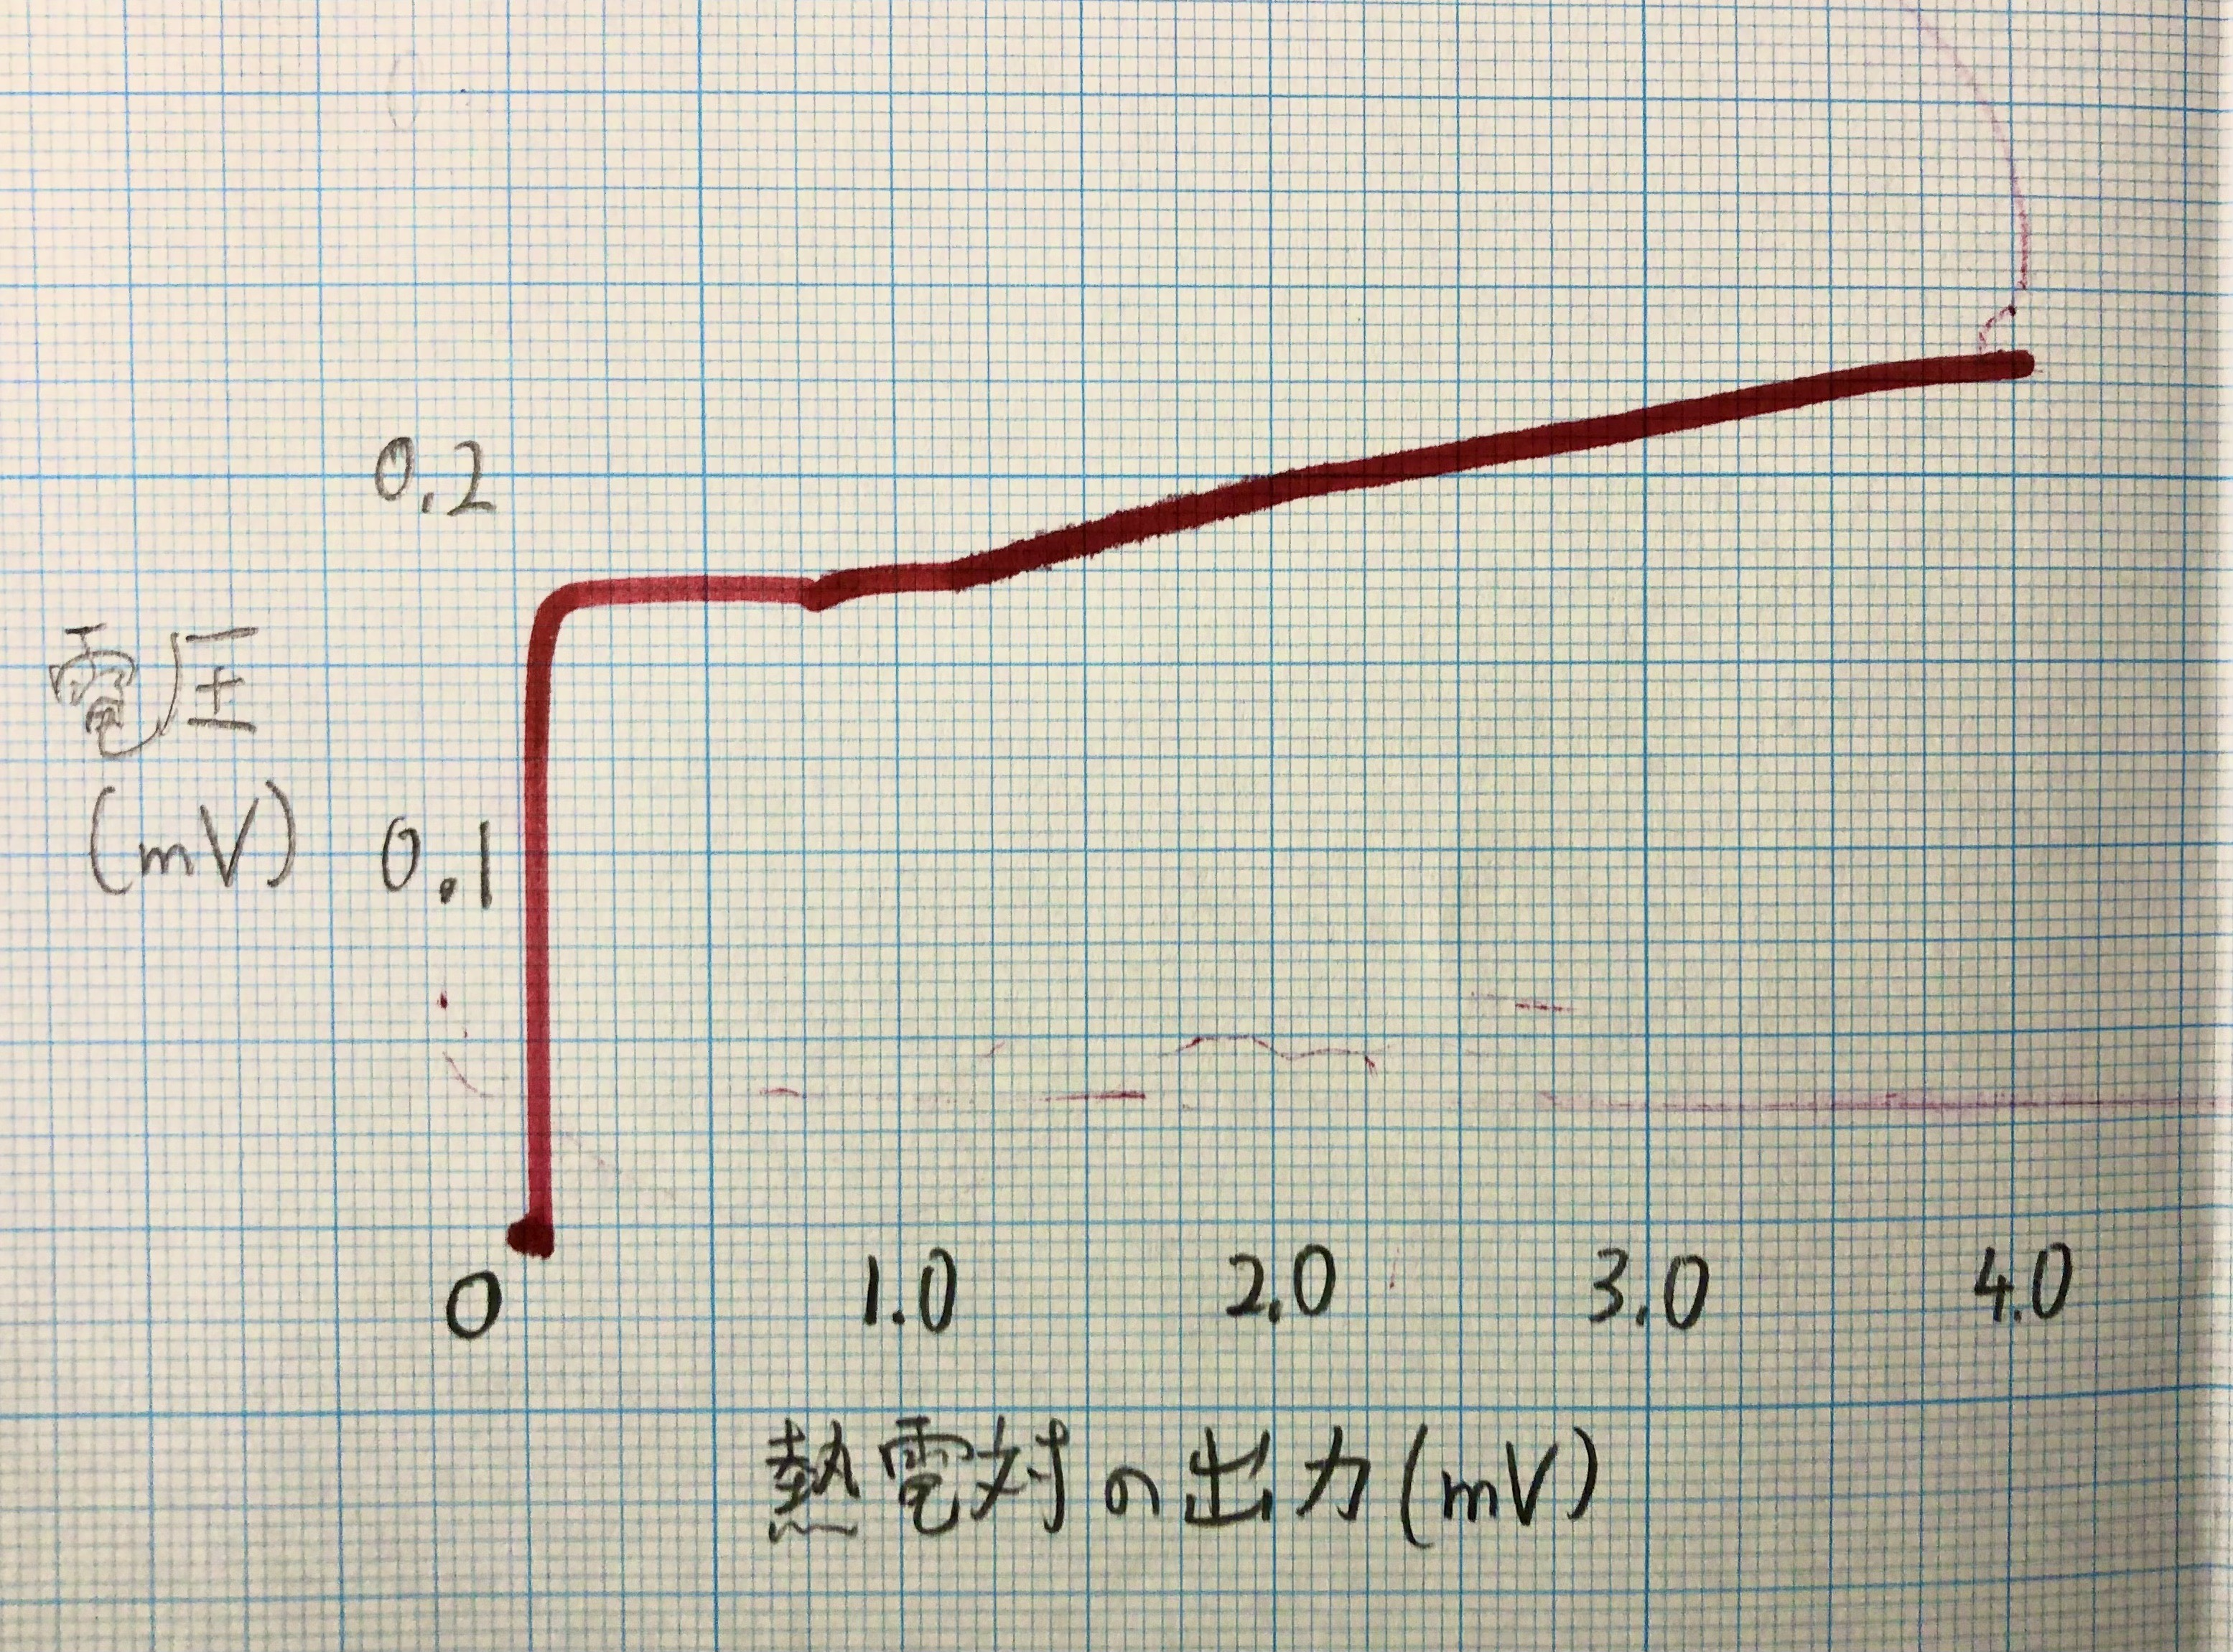
\includegraphics[width=10cm]{./assets/YBCO_resistance.jpg}
  \caption{電気抵抗}
  \label{fig:resistance}
\end{figure}



\subsection{交流帯磁率の測定}
熱電対の出力と電圧の関係は図 \ref{fig:magnetic} のようになった。
\begin{figure}[htbp]
  \centering
  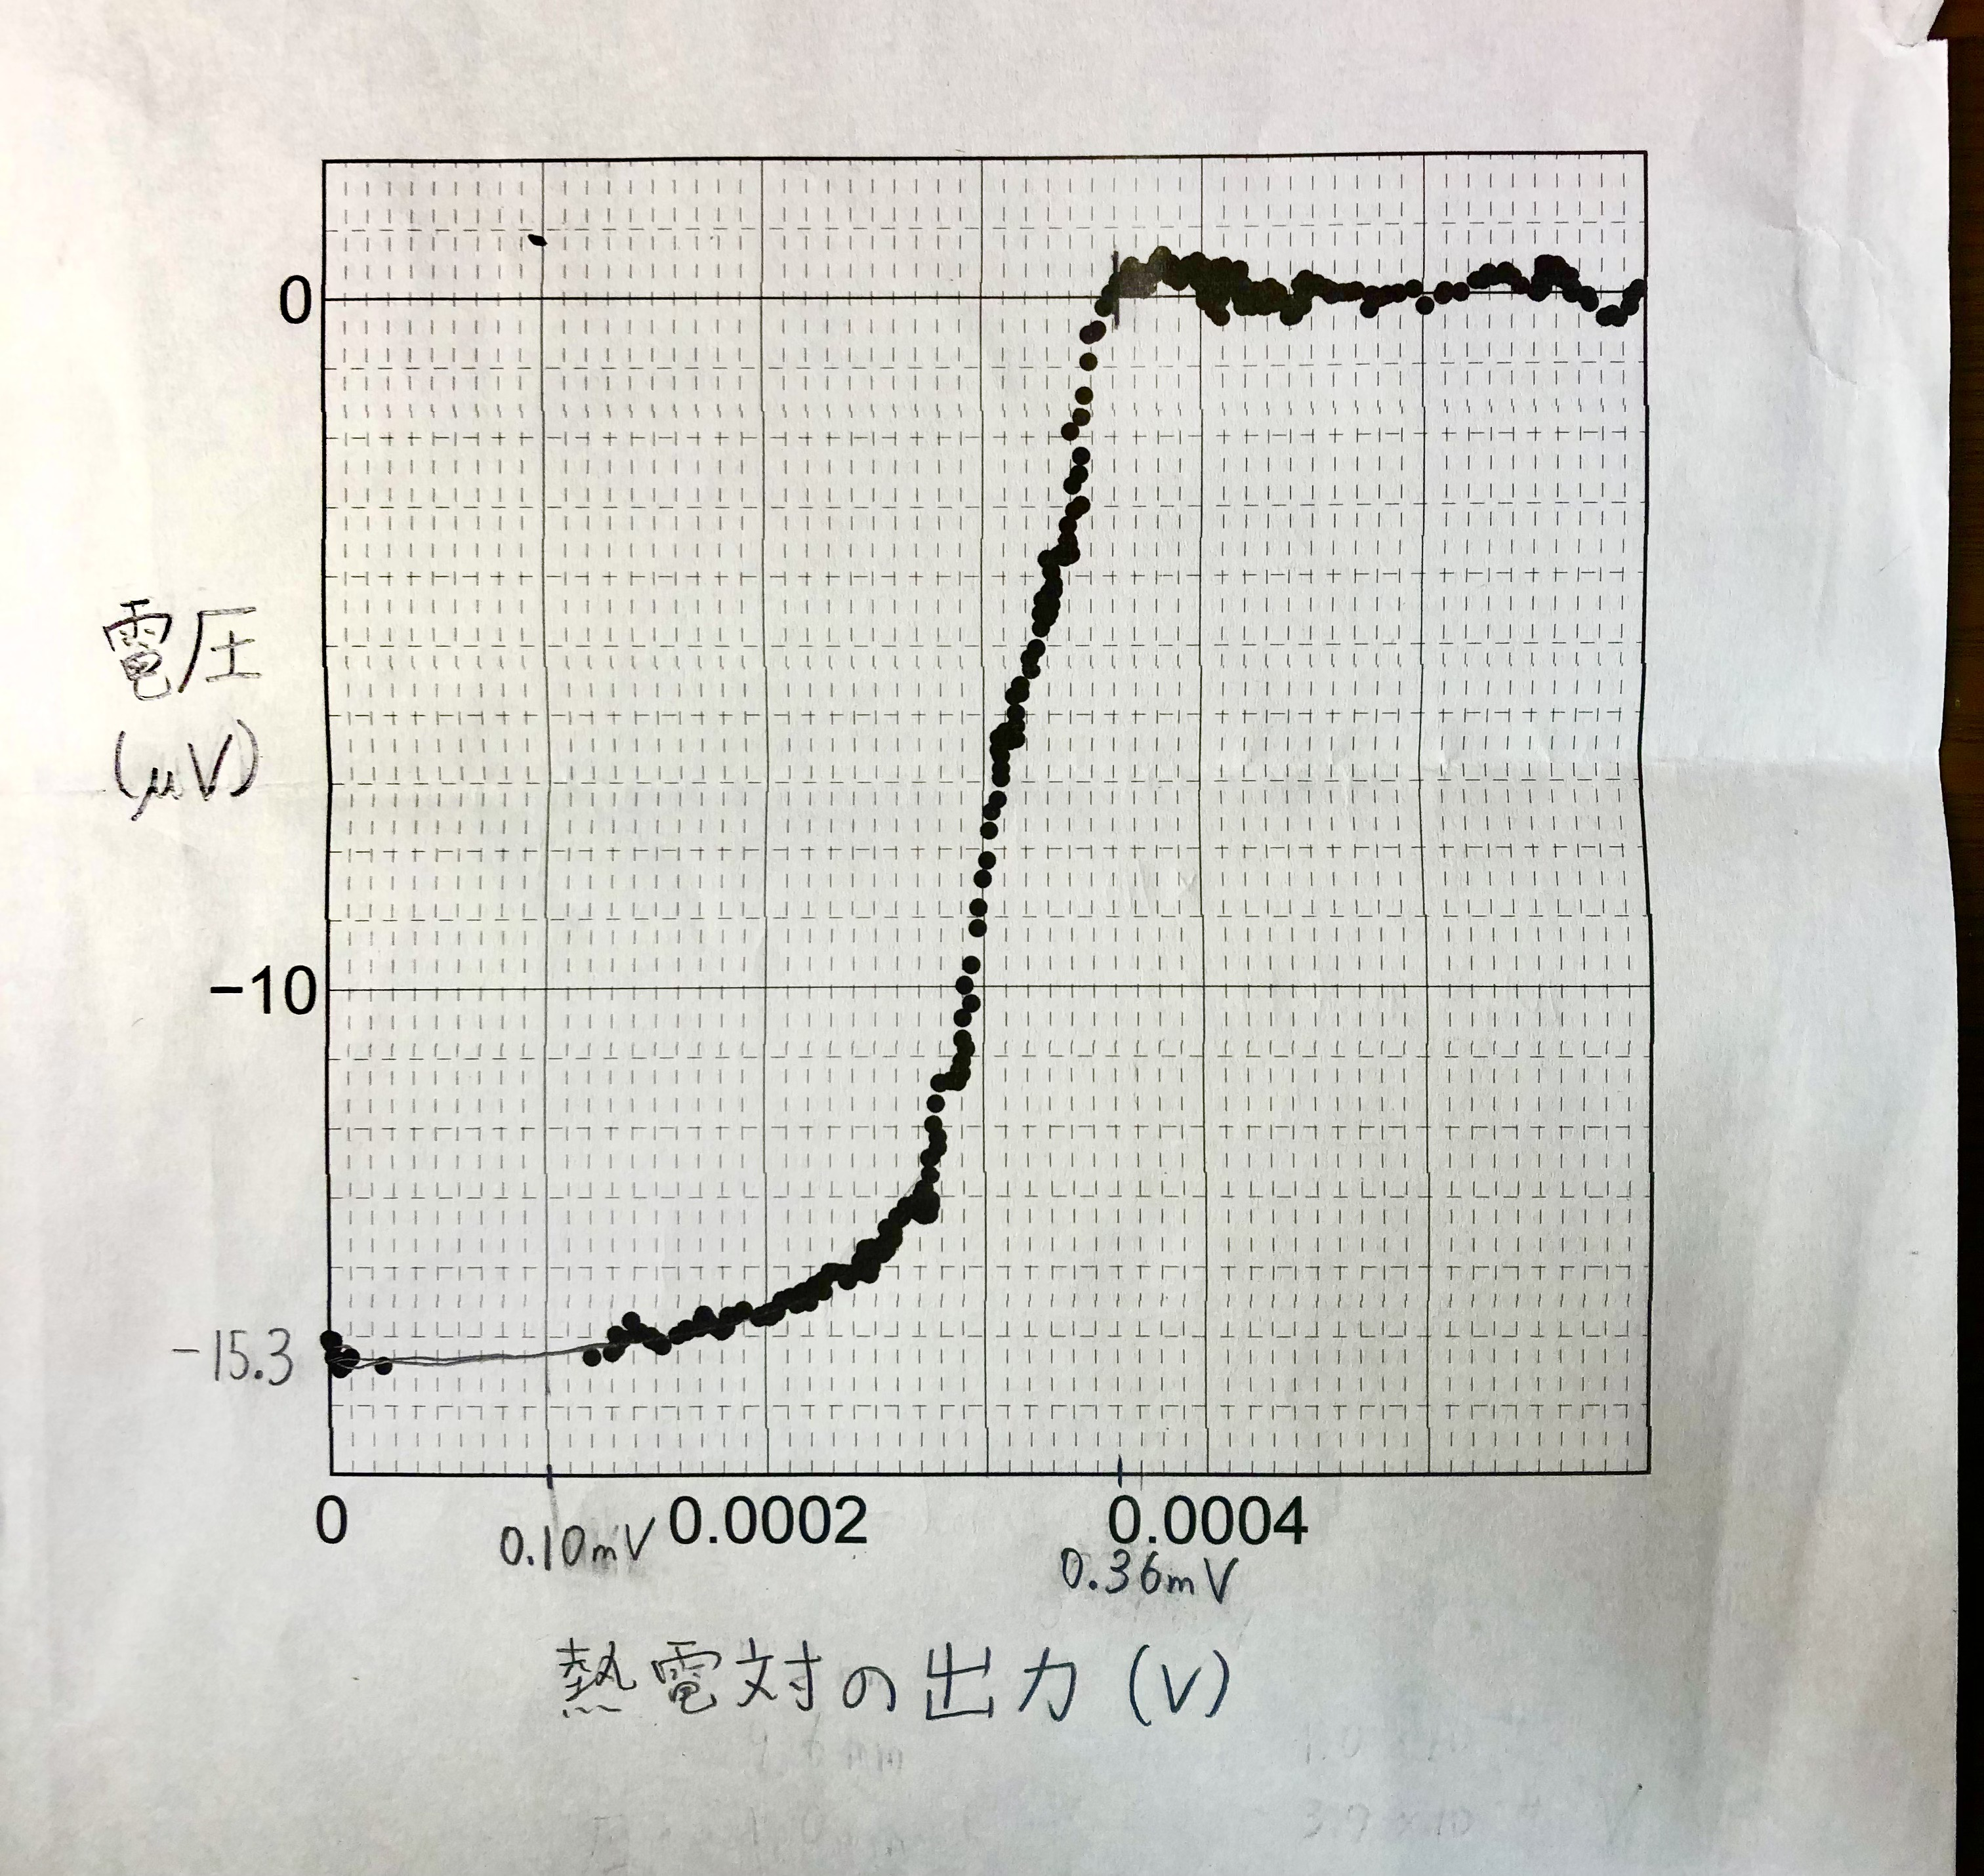
\includegraphics[width=10cm]{./assets/YBCO_magnetic.jpg}
  \caption{交流帯磁率}
  \label{fig:magnetic}
\end{figure}



\section{考察}
\subsection{磁気浮上}
図 \ref{fig:mag1}, 図 \ref{fig:mag2} のような Maxwell の応力が働くことにより試料は浮上している。ピン止め効果については実験結果でまとめたように磁束の向きや場所が固定されることで反発や回転などを引き起こした。


\subsection{X 線回折}
X 線回折を見ると主成分は \ce{YBa2Cu3O7} であることがわかる。また不純物として \ce{Y2BaCuO5} が含まれていることもあり得るが表面に緑色の物質は見えなかった。

帯磁率について超伝導となった体積 $v$ を計算する。
ただしコイルは巻数はどちらも 1000 回であり, コイルは長さ 45 \si{mm}, 直径 20 \si{mm} の円柱形であり, 交流周波数は 110 \si{Hz} とする。
\begin{align}
  V & = 45\si{mm} \times (10\si{mm})^2\pi = 1.414 \times 10^{-5} \si{m^3}                                      \\
  M & = (1.26\times 10^{-6}\si{N/A^2})\times 1000^2 \times V = 1.78\times 10^{-5} \si{H}                       \\
  v & = \frac{-15.3\si{\mu V}}{2\pi \times 110\times (-1\si{mA/V})\times 1\si{V} \times (M/V)} = 17.6\si{mm^3}
\end{align}
すると 67 \% は超伝導化していることがわかる。
これより超伝導体 \ce{YBa2Cu3O7} は 67\% 程度であるとわかる。



\subsection{電気抵抗、交流帯磁率の測定}
電気抵抗については 79-83 \si{K} で超電導となり、抵抗率が転移前 $3.0\times 10^{-5}$ \si{\ohm m} から転移後 0 \si{\ohm m} となった。試料の転移温度と異なるが急激に冷やしてしまった為、温度に関しては熱電対と試料の温度がかけ離れて測定誤差が生まれてしまっていると考えられる。また転移する温度の幅が帯磁率に比べて短いのは端から端まで超伝導の道が出来てしまえば完全に超伝導とならなくても電流が通るからである。

帯磁率に関しては 83-93 \si{K} で超伝導となり、帯磁率が転移前 0 から転移後 $-0.012$ となった。
幅が広いのは完全に超伝導になるまで完全反磁性を示さないことと \ce{YBa2Cu3O7} が酸素欠損の量に依って転移温度が変わる為、均一でなくランダムに酸素欠損していると標準分布に従い、グラフは曲線のようになる。

グラフとしては図 \ref{fig:graph} のようになった。
\begin{figure}[htbp]
  \centering
  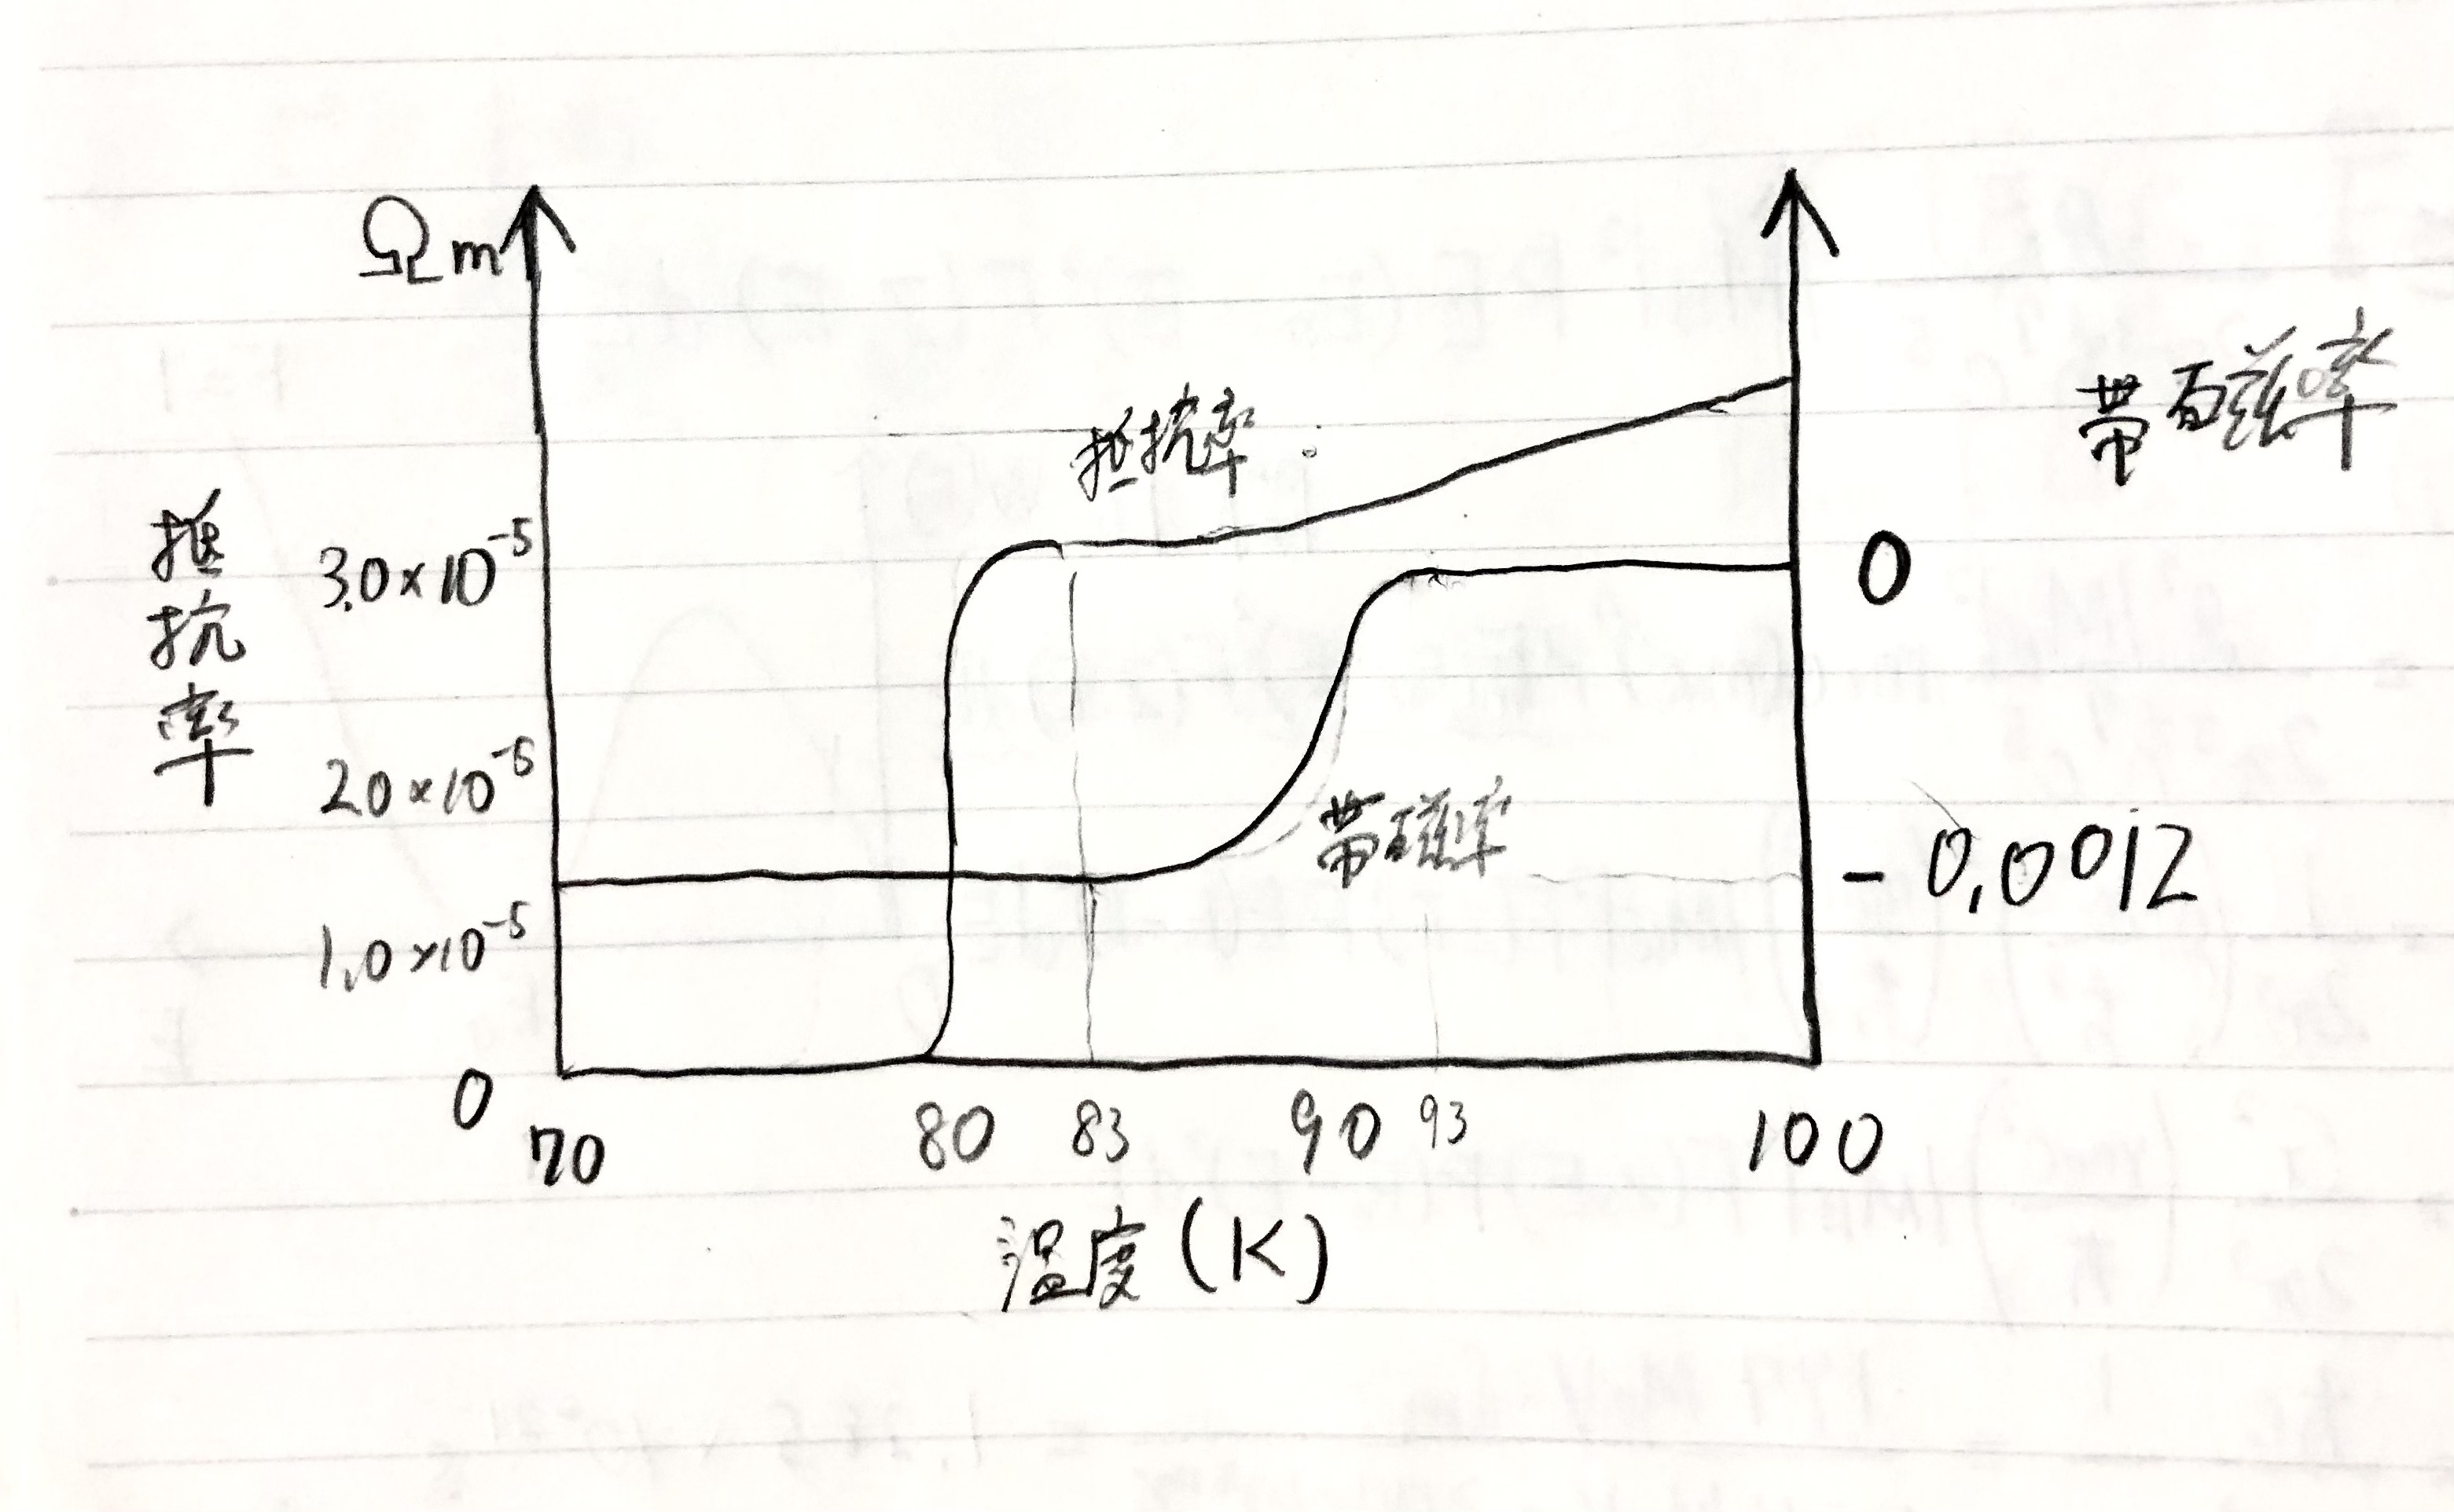
\includegraphics[width=10cm]{./assets/YBCO_graph.jpg}
  \caption{温度と抵抗率、帯磁率の関係}
  \label{fig:graph}
\end{figure}



\section{参考文献}
研究プロジェクト - 東京工業大学 物理学系

\end{document}